\documentclass[12pt]{article}

 \usepackage{graphics}


\usepackage{geometry}
  \geometry{
    a4paper,
    total={6in, 9in},
    top=20mm,
  }

\usepackage{graphicx}
\graphicspath{ {./img/} }

\usepackage{array}
\newcolumntype{P}[1]{>{\centering\arraybackslash}p{#1}}

\usepackage{multirow}
\usepackage{subcaption}
\usepackage{hyperref}

\usepackage{pgfplots}
\pgfplotsset{width=5in,compat=1.9}

\title{Tema 1 Algoritmi genetici \\* Implementare Hill Climbing si Simulated Annealing}
\author{Renghiuc Bianca Elena si Culbece Rose-Marie 2A2}
\date{25.10.2022}

\begin{document}

\maketitle


\section{Introducere}


Raportul nostru contine rezultate, comparatii, concluzii si grafice care scot in evidenta eficienta algoritmilor studiati. Problema presupune gasirea minimului global al unor functii cu dimensiuni diferite. Scopul este observarea algoritmului care ofera rezultate bune pentru imputuri mai mari sau mai mici. Am testat algoritmii folosind urmatoarele patru functii functiile: \href{http://www.geatbx.com/docu/fcnindex-01.html#P89_3085}{\textbf{DeJong's function}}, \href{http://www.geatbx.com/docu/fcnindex-01.html#P150_6749}{\textbf{Schwefel's function}},
\href{http://www.geatbx.com/docu/fcnindex-01.html#P140_6155}{\textbf{Rastrigin's function}} si \href{http://www.geatbx.com/docu/fcnindex-01.html#P204_10395}{\textbf{Michalewicz's function}}. Dupa cum se observa in imaginile de mai jos fiecare functie are un numar diferit de minime pur locale.




\section{Metode}

Hill Climbing si Simulated Annealing sunt algoritmi eficienti, euristici folositi pentru probleme de optimizare matematice. Acestia sunt utili in gasirea optimelor globale. \\*
Am folosit patru metode: {\textbf{Hill Climbing - First Improvement}}, {\textbf{Hill Climbing - Best Improvement}},  {\textbf{Hill Climbing - Worst Improvement}} si {\textbf{Simulated Annealing}}. \\*

Am facut o functie comuna pentru HCFI, HCBI SI HCWI ce ia pe langa restul parametrilor alti doi parametri care vor decide in care versiune din cele trei ne aflam. Pentru a reprezenta numerele am generat un vector de biti ce reprezinta coordonatele punctului curent. Pentru a afla vecinii am negat pe rand fiecare bit din vector. In schimb, pentru a genera un vecin la SA generam o pozitie, negand doar bitul de pe acea pozitie. SA ofera o sansa si solutiilor mai slabe generand o probabilitate, astfel marindu-si domeniul de cautare.


\section{Rezultate}
Mai jos am realizat un tabel pentru fiecare dimensiune studiata. Fiecare celula contine urmatoarele valori in aceasta ordine: valoarea minima, timpul de executie, media valorilor si deviatia standard.


\begin{center}
  \begin{tabular}{ |P{2cm}||P{2.8cm}|P{2.8cm}|P{2.8cm}|P{2.8cm}|  }
      
    \hline
    \multicolumn{5}{|c|}{ Algorithm Result (5) } \\
    
    \hline
      functie & HCFI & HCBI & HCWI & SA \\
    \hline

    De Jong     & \( 1.13687e-10 \) & \(1.13687e-10 \) & \(0.21914 \) & \( 1.15801e-08 \)\\
                & 6m 36s & 7m 32s & 3m 19s & 22s \\
                & \( 1.13687e-10 \) & \( 1.13687e-10 \) &  \( 1.19896 \) &\(1.18321e-08\)\\
                & \( 1.13687e-10 \) & \( 1.13678e-10 \) & \( 1.57886 \)  & \(1.15667\)\\
                \hline
    Schwefel    & \( -2094.91 \) & \( -2094.91 \) & \( -1913.34 \) & \(-2094.91\) \\
                & 9m 52s & 12m 24s & 4m 37s & 26s\\
                & \( -2094.8 \) & \( -2094.91 \) &  \( -1816.04\) & \(-2094.89\)\\
                & \( 4.4632e+06 \) & \( 4.46369e+06 \) & \(2.6618e+06 \) & (2.6608e+06)\\
                \hline
    Rastrigin   & \( 4.51065e-09 \) & \( 4.51065e-09 \) & \( 10.5475 \) & \(4.51065e-09\)\\
                & 5m 21s &  12m 10s &  3m 28s & 27s\\ 
                & \( 0.132669 \) & \( 4.51065e-09 \) &  \( 15.6557 \) & \(2.678e-10\)\\
                & \( 0.0490265 \) & \( 2.06938e-17 \) & \( 13.063 \) & \(0.053954\)\\
                \hline
    Michalewicz & \( -25.8959 \) & \( -3.69888 \) & \( -3.2954 \) & \(-3.69888\)\\
                & 4m 52s & 7m 33s & 2m 30s & 27s \\
                & \( -0.863196 \) & \( -3.69888 \) &  \( -2.94408 \) & \(-3.69888\)\\
                & \( 13.9156 \) & \( 13.9188 \) & \( 8.83487 \) & \( 13.9188 \)\\

    \hline
  \end{tabular}
\end{center}

\begin{center}
  \begin{tabular}{ |P{2cm}||P{2.8cm}|P{2.8cm}|P{2.8cm}|P{2.8cm}| }
      
    \hline
    \multicolumn{5}{|c|}{ Algorithm Result (10) } \\
    
    \hline
      functie & HCFI & HCBI & HCWI & SA\\
    \hline

    De Jong     & \(2.27374e-10\) & \( 2.27374e-10 \) & \( 3.99246 \) & \(1.33266e-07\) \\
                & 40m 15s &  54m 37s & 28m 14s & 45s  \\
                & \( 2.27374e-10 \) & \( 2.9857e-10 \) &  \( 6.5061 \) &  \(2.27374e-10\)\\
                & \( 5.25826e-20 \) & \( 5.25826e-20 \) & \( 16.924 \) & \(2.8954e-20\) \\
                \hline
    Schwefel    & \( -4130.74 \) & \( -4189.51 \) & \( -3630.58 \) & \(-4160.03\)\\
                & 58m 32s & 1h 27m & 23m 8s & 56s\\
                & \( -4112.18 \) & \( -4166.4 \) &  \( -3211.317 \) & \(-41520.48\)\\
                & \( 1.76559e+07 \) & \( 1.76559e+07 \) & \( 5.29618e+06 \) & \(1.87432e+07\) \\
                \hline
    Rastrigin   & \( 1.99004 \) & \( 0.995017 \) & \( 32.247 \) & \(3.23129\) \\
                & 47m 36s & 1h 8m & 31m 14s & 54s\\
                & \( 3.82047 \) & \( 2.46945 \) &  \( 48.3496 \) & \(5.7319\)\\
                & \( 12.1267 \) & \( 4.43286
 \) & \( 139.35 \) & \(17.4815\) \\
                \hline
    Michalewicz & \( -8.61317 \) & \( -8.6432 \) & \( -5.06779 \) & \(-8.59603\)\\
                & 45m 17s &  1h 12m & 29m 47s & 48s \\
                & \( -8.61317 \) & \( -7.131895 \) &  \( -4.49717 \) & \(-8.5402\)\\
                & \( 34.0163 \) & \( 45.0906 \) & \( 20.6067 \) & \(42.6825\) \\

    \hline
  \end{tabular}
\end{center}

\begin{center}
  \begin{tabular}{ |P{2cm}||P{2.8cm}|P{2.8cm}|P{2.8cm}|P{2.8cm}|}
      
    \hline
    \multicolumn{5}{|c|}{ Algorithm Result (30) } \\
    
    \hline
      functie & HCFI & HCBI & HCWI & SA \\
    \hline

    De Jong     & \( 6.82121e-10 \) & \( 6.82121e-10 \) & \( 51.3112 \) & \(0.00135782\) \\
                & 6h 3m & 6h 41m & 5h 56m & 2m 36s\\
                & \( 8.3257e-10 \) & \( 8.3257e-10 \) &  \( 72.972082 \) & \(0.145921\)\\
                
                \hline
    Schwefel    & \( -11122.1 \) & \( -11807.9\) & \( -7148.69 \) & \(-11656.1\)\\
                & 7h 43m & 8h 36m & 5h 57m & 2m 21s \\
                & \( -11094.3 \) & \( -11605.7 \) &  \( -6238.52 \) & \(-11576.4\)\\
                
                \hline
    Rastrigin   & \( 33.2081 \) & \( 23.0617 \) & \( 84.493 \) & \(31.296\)\\
                & 6h 12m & 8h 35m & 6h 2m & 2m 52s\\
                & \( 35.10694 \) & \( 28.0617 \) &  \( 93.73304 \) & \(36.37624\)\\

                \hline
    Michalewicz & \( -25.8959 \) & \(-26.4804 \) & \( -8.46187 \) & \(-24.9721\)\\
                & 4h 40m & 6h 37m & 5h 48m & 3m 10s\\
                & \( -25.8959 \) & \( -26.4804 \) &  \( -7.46187 \) & \(-22.9721\)\\

    \hline
  \end{tabular}
\end{center}

In acest grafic se poate observa variatia timpului de executare pe masura ce valoarea inputului (numarul de componente) creste. Astfel, am ales functia Rastrigin. 


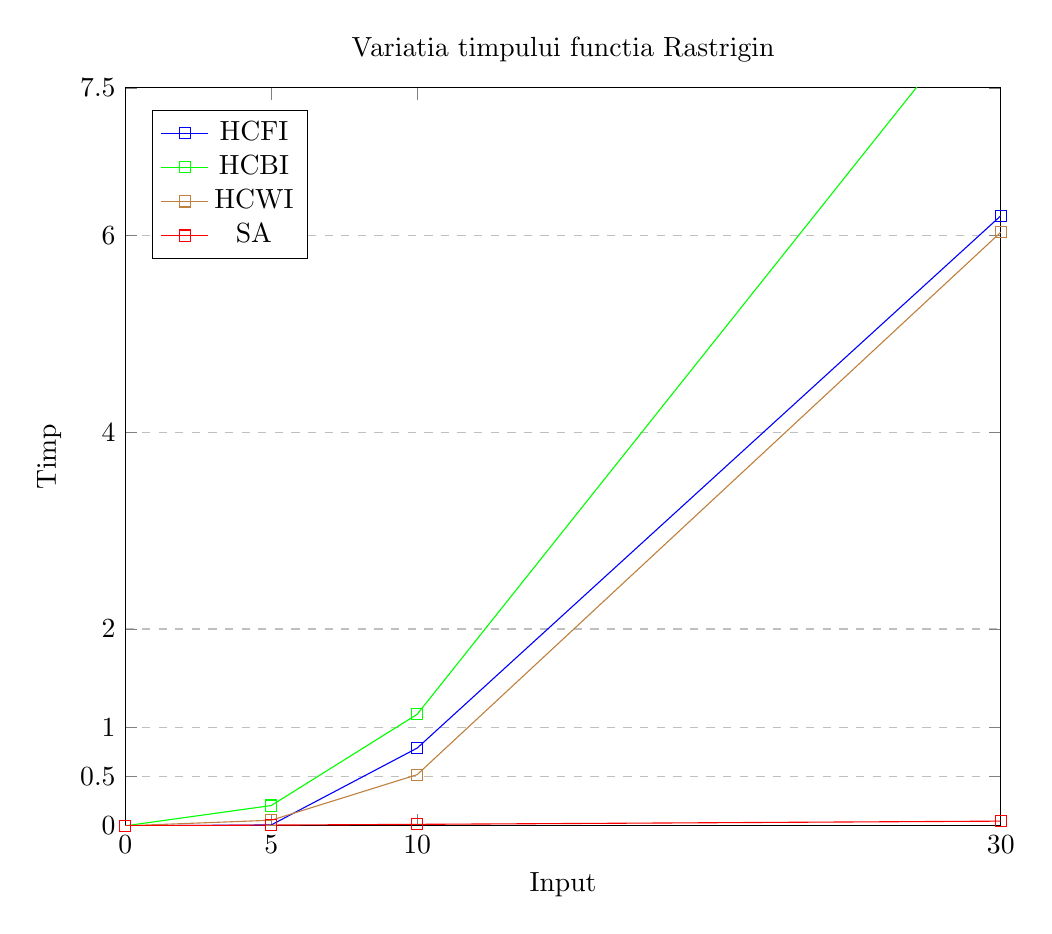
\begin{tikzpicture}
  \begin{axis}[
      title={Variatia timpului functia Rastrigin },
      xlabel={Input},
      ylabel={Timp},
      xmin=0, xmax=30,
      ymin=0, ymax=7.5,
      xtick={0,5,10,30},
      ytick={0,0.5,1,2,4,6,7.5},
      legend pos=north west,
      ymajorgrids=true,
      grid style=dashed,
  ]
  
  \addplot[
      color=blue,
      mark=square,
      ]
      coordinates {
      (0,0)(5, 0.0089)(10, 0.79)(30, 6.2)
      };
      \addlegendentry{HCFI}
      
  \addplot[
      color=green,
      mark=square,
      ]
      coordinates {
      (0,0)(5, 0.206)(10, 1.1333)(30, 8.58)
      };
      \addlegendentry{HCBI}

   \addplot[
      color=brown,
      mark=square,
      ]
      coordinates {
      (0,0)(5, 0.057)(10, 0.52)(30, 6.033)
      };
      \addlegendentry{HCWI}

  \addplot[
      color=red,
      mark=square,
      ]
      coordinates {
      (0,0)(5, 0.0075)(10, 0.015)(30, 0.0477)
      };
      \addlegendentry{SA}
      
  \end{axis}
\end{tikzpicture}


Se observa in graficul de mai sus ca imputul are un impact major asupra algoritmului HC. In schimb, timpul algoritmului SA nu se schimba semnificativ.

\section{Comparatii}
Mai departe vom vedea care sunt diferentele dintre algoritmi. HC alege mereu un vecin mai bun ( chiar daca este primul -FI, cel mai bun din cei mai buni -BI sau cel mai rau din cei mai buni -WI ). In schimb SA poate alege un vecin mai rau daca se genereaza o probabilitate cat mai mica, astfel marindu-si raza de cautare. Dintre cei 2 algoritmi se observa ca SA are un timp de rulare mult mai bun dar, pe masura ce creste dimensiunea, HCBI va da rezultate mai bune decat SA.


\section{Concluzie}
In concluzie, algoritmii euristici ne ajuta sa rezolvam destul de eficient si rapid, probleme pe care algoritmii deterministi nu le pot rezolva pentru imputuri mari. Testand cei patru algoritmi euristici enumerati la inceput putem ajunge la concluzia ca SA este mult mai bun. Desi, pentru valori mari se indeparteaza putin de optim acesta este foarte rapid. Pe de alta parte, HC da rezultate mai bune dar, intr-un timp mult mai lung.

\begin{thebibliography}{9}
  \bibitem{}
    \url{https://towardsdatascience.com/how-to-implement-the-hill-climbing-algorithm-in-python-1c65c29469de}
  \bibitem{}
    \url{https://en.wikipedia.org/wiki/Hill_climbing}
  \bibitem{}
    \url{https://en.wikipedia.org/wiki/Simulated_annealing}
  \bibitem{}
    \url{https://hal.archives-ouvertes.fr/hal-01962309/document}
  \bibitem{}
    \url{https://profs.info.uaic.ro/~eugennc/teaching/ga/}
  \bibitem{}
    \url{http://www.geatbx.com/docu/fcnindex-01.html#P150_6749}
  \bibitem{}
    \url{http://www.geatbx.com/docu/fcnindex-01.html#P140_6155}
  \bibitem{}
    \url{http://www.geatbx.com/docu/fcnindex-01.html#P204_10395}
  \bibitem{}
    \url{http://www.geatbx.com/docu/fcnindex-01.html#P89_3085}
  \bibitem{}
    \url{https://machinelearningmastery.com/simulated-annealing-from-scratch-in-python/}
  \end{thebibliography}  
  


\end{document}
